\documentclass{beamer}
\usepackage{beamerthemesplit}
\usepackage{tikz}
\usepackage{ocgx2}
\usepackage{amsmath,amsthm,amssymb,amscd, graphicx,bbm,xcolor}
\usepackage{array}
\usepackage{etoolbox}
\usepackage{mathtools}
\usepackage{subfig}
\usepackage{multirow}
\DeclareMathOperator{\E}{E}
\DeclareMathOperator{\V}{Var}
\DeclareMathOperator{\cov}{Cov}
\newcommand{\h}[1]{\hat{#1}}
\newcommand{\I}{I}
% \newcommand{\partiall}[1]{\frac{\partial}{\partial #1}}
% \newcommand{\gm}{\theta}
% \newcommand{\E}{E}
\renewcommand{\P}{P}
% \newcommand{\mean}[1]{\overline{#1}}
% \newcommand{\sel}[1]{#1^*}
% \newcommand{\biasratio}{b}% {$(E|S_1-S_2|)^2/\E(S^2)$}
\newcommand{\cind}{\perp \!\!\! \perp}
\newcommand{\aucindiv}{\theta_{11}}%{\AUC}
\newcommand{\aucpop}{\theta_{12}}%{\AUC_{\cind}}
\newcommand{\aucindivhat}{\hat{\theta}_{11}}%{\AUC}
\newcommand{\aucpophat}{\hat{\theta}_{12}}%{\AUC_{\cind}}
\newcommand{\kernel}{\psi}
\newcommand{\Kernel}{\psi}
\newcommand{\B}{B}
% \newcommand{\W}[1]{X_{#1},Y_{#1}}
\newcommand{\W}[1]{W_{#1}}
\newcommand{\bnd}{a}
% \renewcommand{\V}{c_{00}}
\newcommand{\seqspace}{V}%{c_{00}}
\renewcommand{\d}{\phi}
\newcommand{\Pind}{P_{\cind}}
\newcommand{\A}[1]{P(A^{(n)}_{#1})}
% \newtheorem{theorem}{Theorem}
\newtheorem{proposition}[theorem]{Proposition}
% \newtheorem{lemma}[theorem]{Lemma}
% \newtheorem{corollary}[theorem]{Corollary}

\setbeamertemplate{navigation symbols}{}
\newcommand{\PreserveBackslash}[1]{\let\temp=\\#1\let\\=\temp}
\newcolumntype{C}[1]{>{\PreserveBackslash\centering}p{#1}}
\graphicspath{{../manuscript/figs/}{../../1/ms/}}
% \graphicspath{{./figs/}}
\makeatletter
\def\input@path{{../manuscript/}}
% \graphicspath{{../../1/ms/}{../../1/ms/figs}}
% \graphicspath{{./figs/}}
\makeatother
\usetikzlibrary{calc}
\mathtoolsset{showonlyrefs=true}
\newtoggle{speaktoggle}
\togglefalse{speaktoggle}
\newcommand{\speak}[1]{
  \iftoggle{speaktoggle}{
    {\tiny{\textcolor{red}{speak: #1}}\normalsize}
  }
  {}
}
% \makeatletter
% \def\input@path{{../manuscript/}}
% % or: \def\input@path{{/path/to/folder/}{/path/to/other/folder/}}
% \makeatother\setbeamertemplate{footline}[frame number]

\title{The Personalized and Population AUCs}
% \author{Haben Michael}
\date{}

\AtBeginSection[] 
{
  \begin{frame}<beamer>
    \frametitle{Outline} 
    \tableofcontents[currentsection]  
  \end{frame}
}

\begin{document}



\begin{frame}
  \titlepage
\end{frame}




% 1. intro
% motivating example [copy old]
% define auc [copy old]
% need generalization for this type of data--vectors of obs, and dependence pairwise bw case and control
% example applications

% 2. generalization of auc to cluster data

% let xymn be a random vector with joint distr...
% let psi denote the auc between control cluster i and case cluster j
% a. with xymn and xymn being two ndependent draws from P, we define the population auc as:

% this is the most commonly used generalization to clusters. analogues show up in the literature.

% b. individualize trt--natl acad quote

% c. present personalized and population auc side by side. the individualized auc is:
% cc. ``Both the population and personalized AUC, like the usual AUC, are bounded between 0
% and 1, 1
% 2 represents poor discrimination, and distance from 1
% 2 represents increasing discrim-
% ination. However, they describe distinct measures of discrimination. It is possible for one
% to be informative and therefore far from 1/2, while the other is non-informative, or close to
% 1/2. Whereas the personalized AUC is the AUC of a typical cluster, the population AUC
% is, setting aside ties in the data, the probability that a typical control observation in the
% population is less than a typical case observation.''
% d. propositions for population auc

% e. estimators. individual auc is just an iid average.  pop est is
% theta12(empirical). a little more complicated to analyze. previous analysis [obu] uses ratio estimator, mayb emention ends up with an asy variance estimator nearly same as jk and cite other work. not quite a
% u-statistic. mention a benefit of this reserach was to clarify the
% statistical model and asymptotics of the pop auc, which already shows
% up in similar forms. cavest that m and n ge 0.

% 3. illustrations. mention motivation was many biostaticians intuited that pop auc as more informative. on some level recognized there is an indvidual auc. goal of this work is to investigate when this is true, but also when they disagree.
% a. simpsons paradox examples
% a1. let the distribution of --
% a2. the individ auc is-- [note simplifaction for later]. the pop auc is --
% a3. [images]
% b. causal inference examples

% 4. simplifications when the cluster values are independent of the cluster sizes
% a. as expected, if the within cluster auc order relation is constant for all pairs, can reduce to the m=n=1 case. [counter example when m,n not independent of x,y]
% b. the population auc may bound the individual auc
% b1. illustrate the interplay bw joint distr and marginals, in the m=n=1 case
% b2. [give picture]


% simulations
% fpr
% power

% data application


\section{Introduction}
\begin{frame}
  \centering
  A motivating example
  \medskip
  \begin{columns}
    \begin{column}{.3\textwidth}
      Data: The Yale Prospective Longitudinal HIV Cohort
      \vspace{.2in}
      
      Problem: Evaluate CD4 as a predictor of blip status
    \end{column}
    \begin{column}{.7\textwidth}
      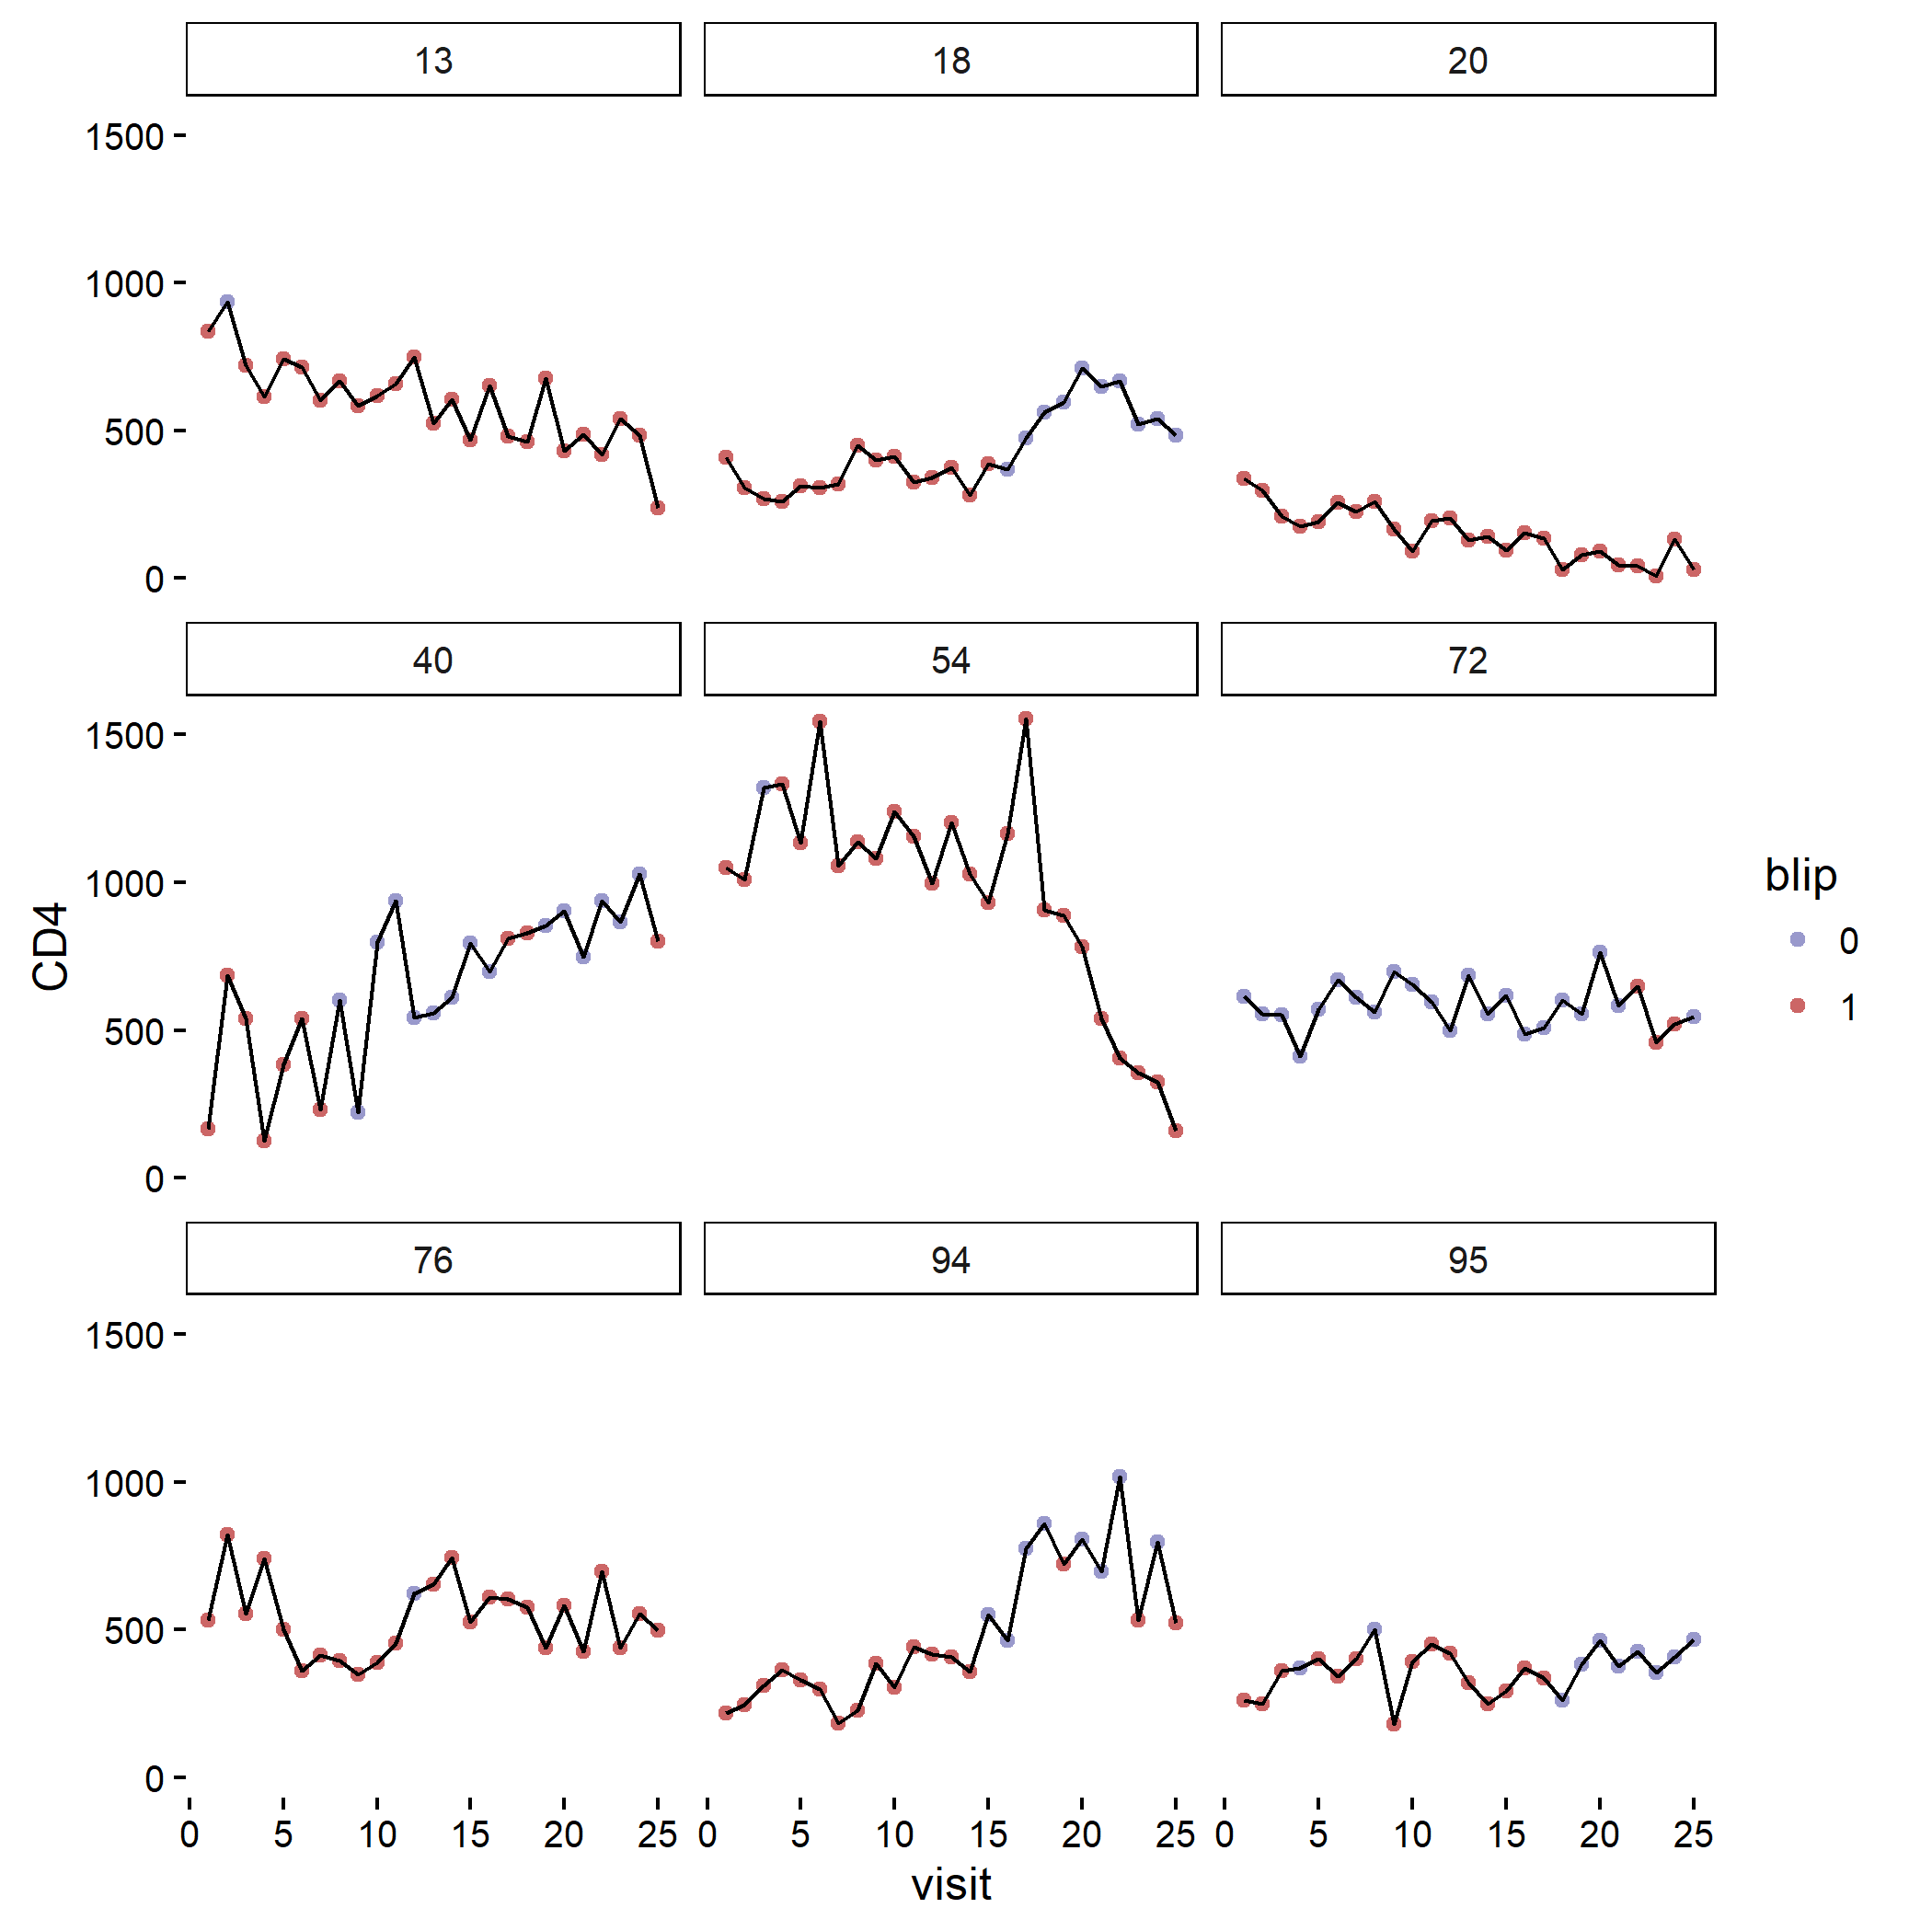
\includegraphics[width=\textwidth]{fig5.png}
    \end{column}
  \end{columns}
  
  % motivating example -- 
  % 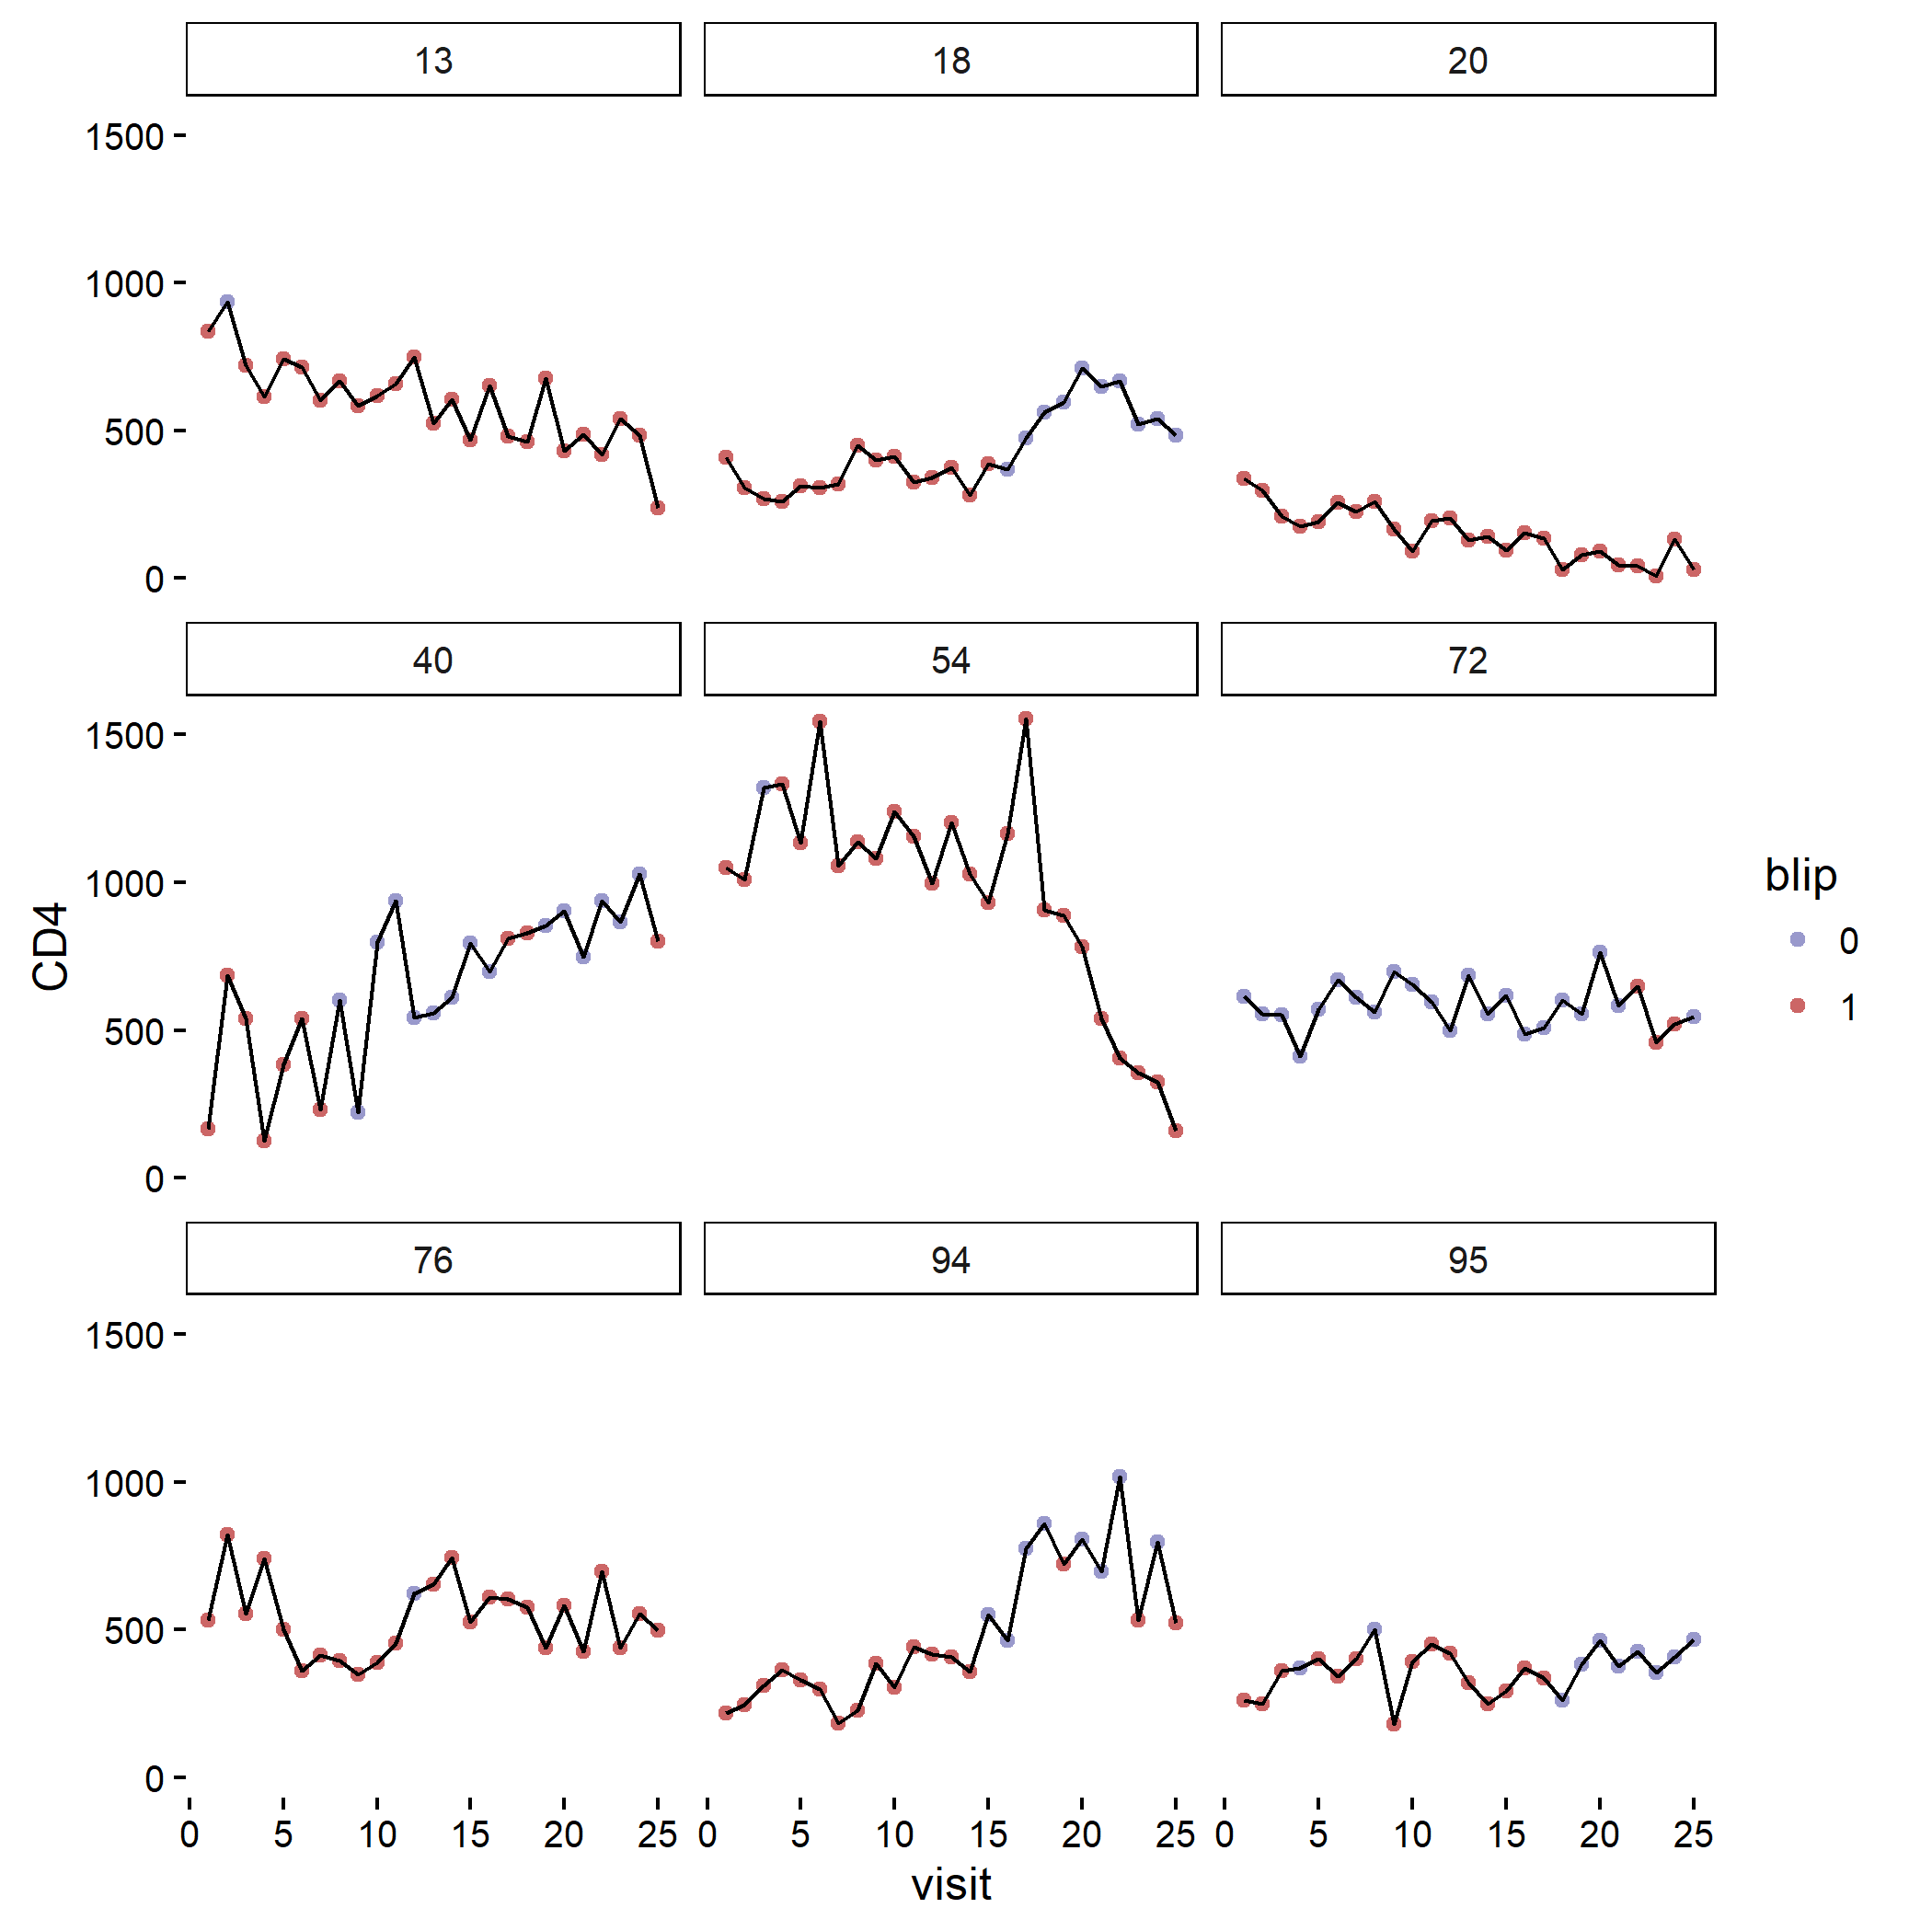
\includegraphics[scale=.4]{fig5.png}
\end{frame}
\begin{frame}
  \centering
  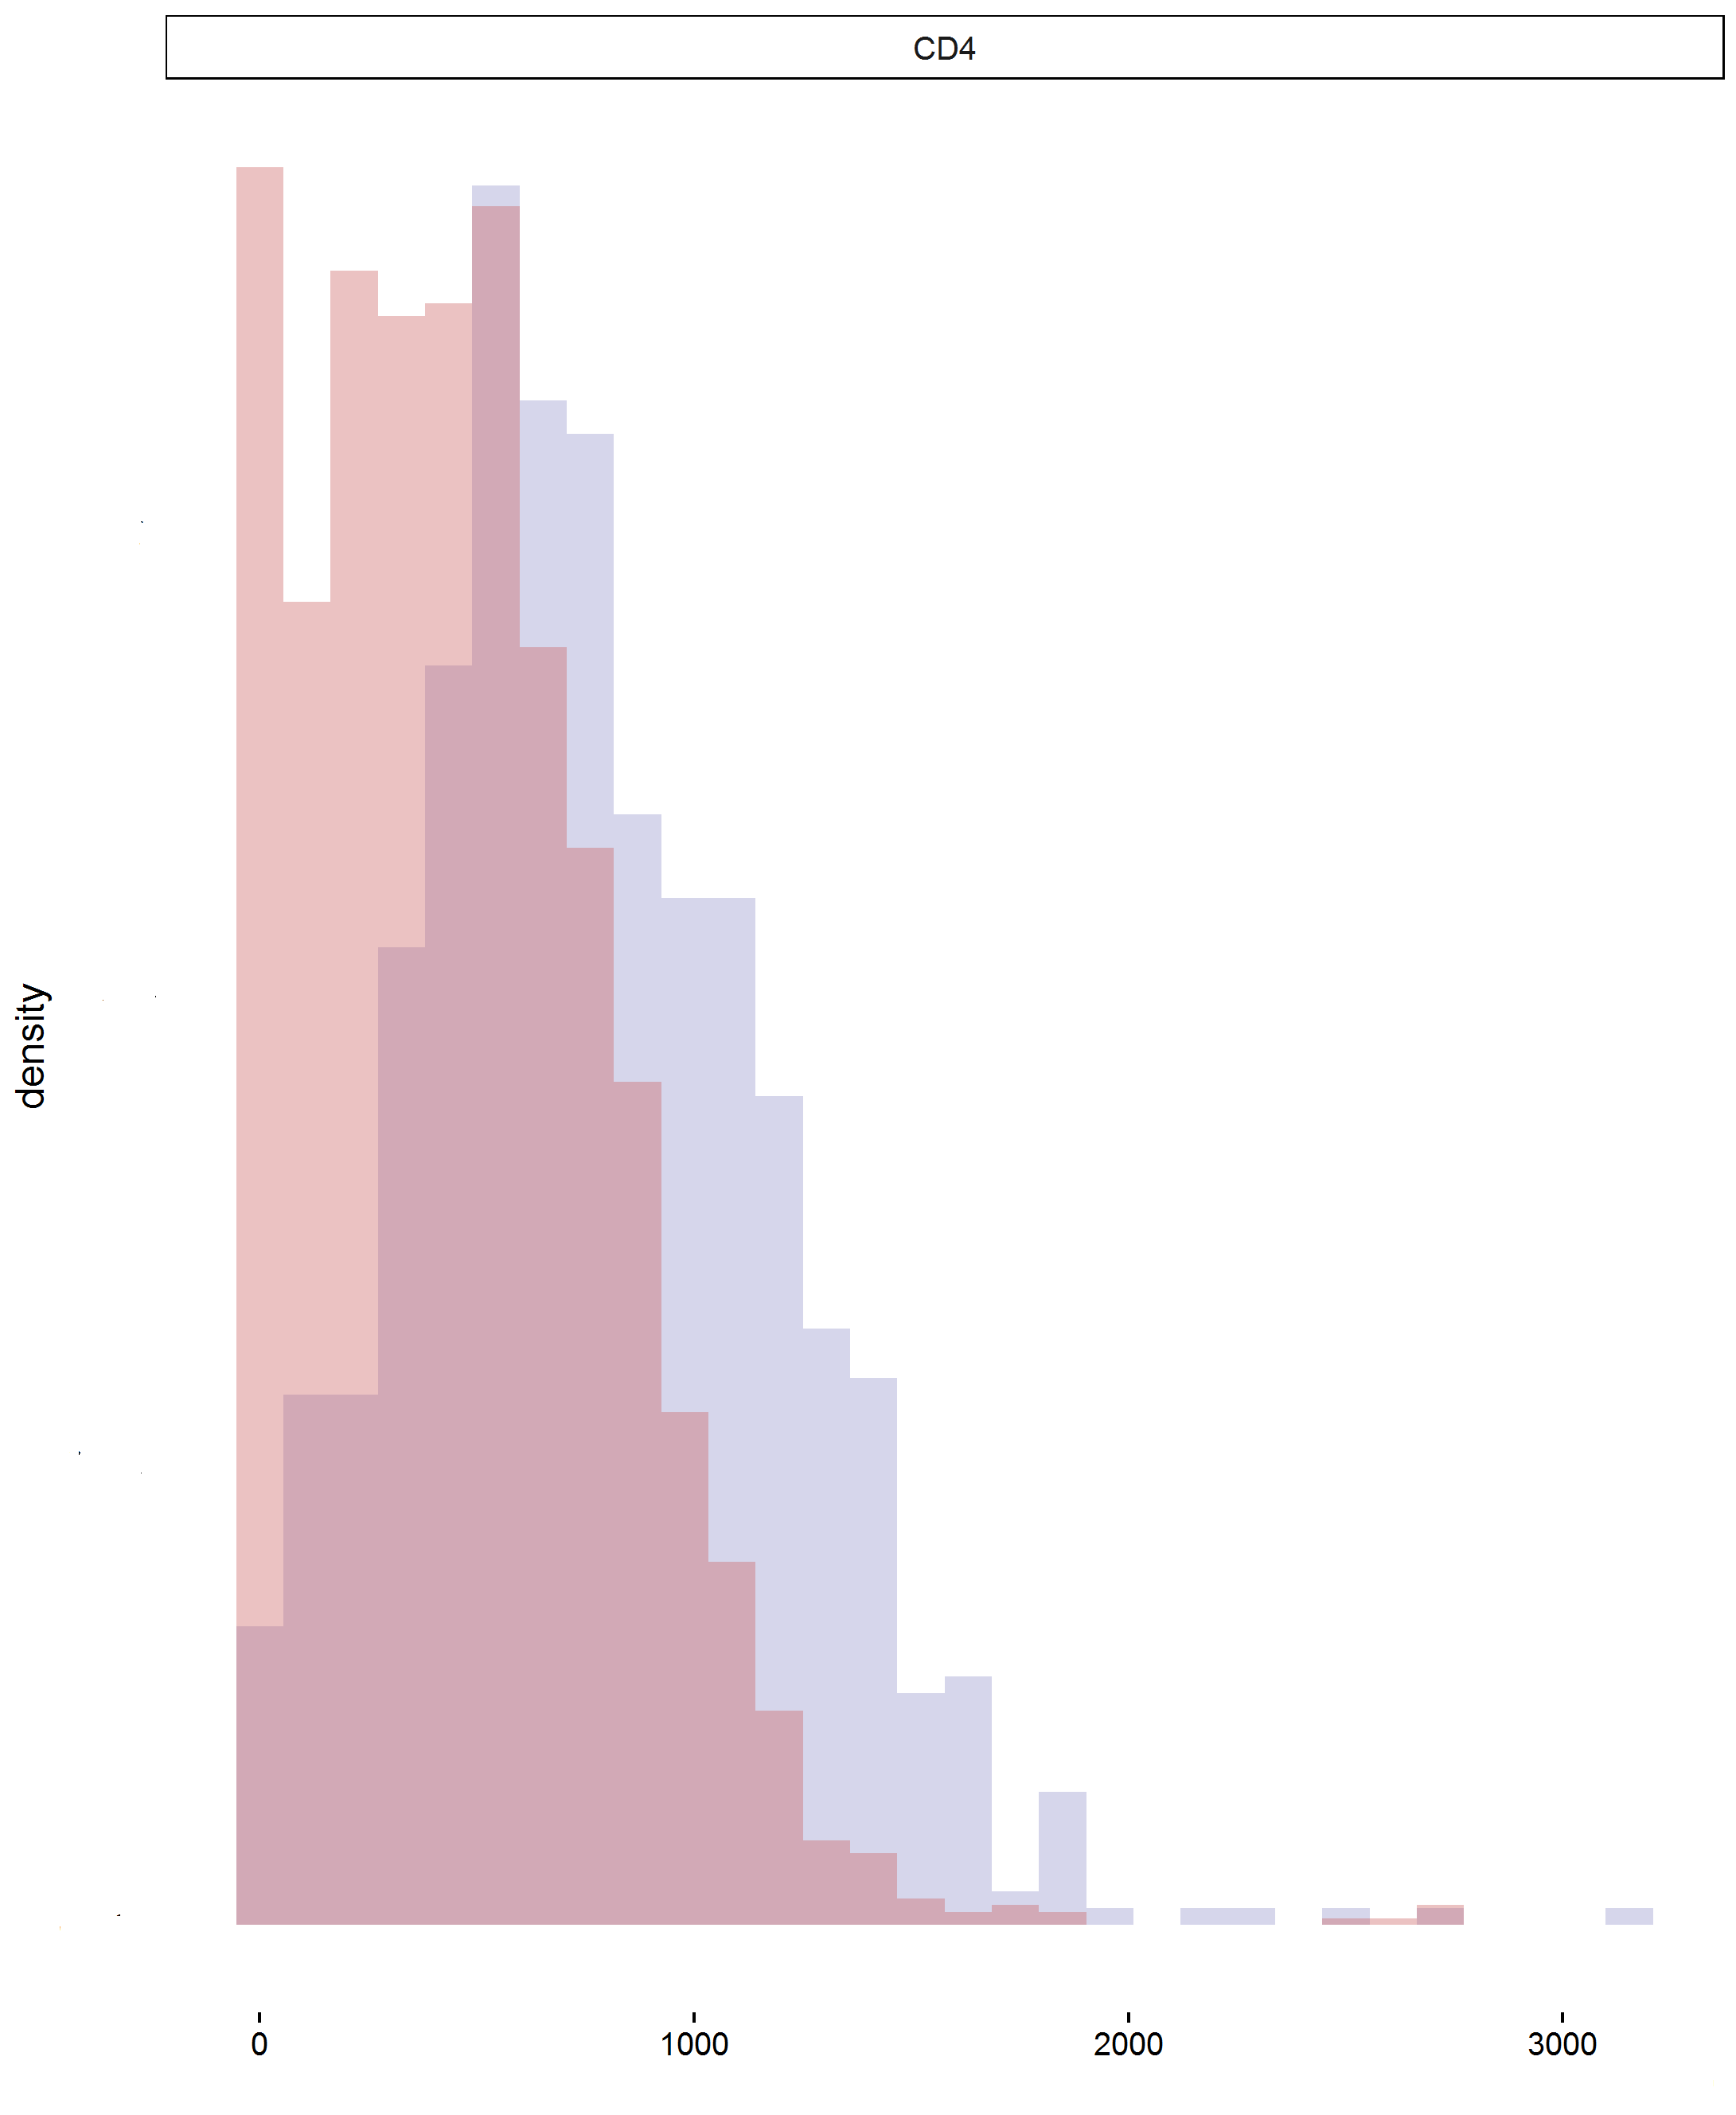
\includegraphics[scale=.22]{fig4.png}
\end{frame}
\begin{frame}
  \begin{columns}
    \begin{column}{.5\textwidth}
  \begin{tabular}{c | c | c}
    & control & case\\
    \hline&&\\
    obs. \# 1 & $X_1$ & \\
    \vdots & \vdots & \\
    obs. \# k & $X_{k}$ &\\
      obs. \# k+1 &  & $Y_{k+1}$\\
     \vdots & & \vdots\\
    obs. \# \I &  & $Y_{\I}$\\
  \end{tabular}
\end{column}
\begin{column}{.5\textwidth}
  The AUC is the probability that an observation drawn from a
  negative/control/non-diseased subject is less than an independent
  observation from a positive/case/diseased subject.
  % $$\text{AUC}=\P(X < Y)=\E(F_X(Y))$$
  % $$\widehat{\text{AUC}}=\frac{1}{k(\I-k)}\sum_{i,j}\{X_i<Y_j\}$$
  $$\theta(P)=\P(X < Y)=\E(F_X(Y))$$
  $$\hat{\theta}(\vec X,\vec Y)=\frac{1}{k(\I-k)}\sum_{i,j}\{X_i<Y_j\}$$
\end{column}
\end{columns}
\end{frame}


\begin{frame}
  We wish to extend the AUC to clusters



  \begin{itemize}
  \item markers: longitudinal measurements of tumour antigens (CEA,
    CA15-3, TPS), response: progression/non-progression of breast
    cancer (Emir 2000)

  % \item markers: two measurements of the distortion product
  %   otoacoustic emissions taken from the left and right ears of each
  %   patient, response: neonatal hearing impairment (Wu 2019)

  % \item markers: longitudinal measurements of levels of vascular
  %   enothelial growth factor, % and a soluble fragment of Cytokeratin 19
  %   response: progression/non-progression of non-small cell lung
  %   cancer (Wu, Wang 2011)

  \item markers: how long an officer detains a suspect (clustered by
    officer), response: non-Black (``control'') or Black (``case'')
    suspect status (Ridgeway 2006)
   \end{itemize}
 \end{frame}

 \begin{frame}
  \centering
  \begin{tabular}{c | c | c}
    & control & case\\
    \hline&&\\
    obs. \# 1 & $(X_{11},\ldots,X_{1m_1})$ & $(Y_{11},\ldots,Y_{1n_1})$\\
    \vdots & \vdots & \vdots\\
    obs. \# \I & $(X_{\I1},\ldots,X_{\I m_{\I}})$ & $(Y_{\I1},\ldots,Y_{\I n_{\I}})$\\
  \end{tabular}
 \begin{itemize}
  \item     Let $(X,Y,M,N)$ be a random vector
    with joint distribution denoted $\P$
  \item $X$ and $Y$ are vectors of control and case observations of lengths $M$ and $N$
    % such that $X$ and $Y$ are sequences and $M$ and $N$ are counting numbers.%$X$ is a vector of length $M$
    % and $Y$ is a vector of length $N$, where $M$ and $N$ are counting
    % numbers.
    % \begin{gather}
    %   \begin{aligned}\label{model:cluster auc}
    %     &(X,Y,M,N) \sim \P\\
    %     &X=(X_1,X_2,\ldots)\in\mathbb{R}^\mathbb{N}, Y=(Y_1,Y_2,\ldots)\in\mathbb{R}^\mathbb{N}\\
    %     &M,N \in 1,2,3,\ldots .
    %   \end{aligned}
    % \end{gather}
  \end{itemize}
  % think of x and y as vectors of length m and n
\end{frame}

\begin{frame}
  With $(X_1,Y_1,M_1,N_1)$ and $(X_2,Y_2,M_2,N_2),$ being two independent draws from $P$, we define the population AUC as
  \begin{gather}
    \begin{aligned}
      &\aucpop(\P)=\frac{\E\hat{\theta}(X_1,Y_2)}{\E(M_1)\E(N_2)}
      = \frac{1}{\E(M_1)\E(N_2)}\E\left( \sum_{i=1}^{M_1}\sum_{j=1}^{N_2}\{X_{1i}<Y_{2j}\}\right)\\
      &(X_1,Y_1,M_1,N_1),(X_2,Y_2,M_2,N_2) \overset{\text{IID}}{\sim} \P.
    \end{aligned}
  \end{gather}
  % this parameter/the model appears to be implied by what the applied researchers have in mind
\end{frame}

\begin{frame}
  \begin{itemize}
  \item     the medical field has lately focused on
    personalizing treatment
  \item For example, in 2018 the National Academy of Medicine concluded: ``The
    individuality of the patient should be at the core of every treatment
    decision. One-size-fits-all approaches to treating medical conditions
    are inadequate; instead, treatments should be tailored to individuals
    . . .''
  \end{itemize}
\end{frame}

\begin{frame}
 Besides the population AUC
$$      \aucpop(\P)=\frac{\E\hat\theta(X_1,Y_2)}{\E(M_1)\E(N_2)}
$$
we define the personalized AUC as:
\begin{align}
  \aucindiv(\P)=\E\left(\frac{\hat\theta(X_1,Y_1)}{M_1N_1} \right)
  = \E\left(\frac{ \sum_{i=1}^{M_1}\sum_{j=1}^{N_1}\{X_{1i}<Y_{1j}\}}{M_1N_1} \right)\\.
  \label{defn:aucindiv}
\end{align}

(Definition requires $M>0,N>0$.)


\end{frame}

\begin{frame}
  \begin{itemize}
\item Both the population and personalized AUC, like the usual AUC, are bounded between 0
and 1, $1/2$ represents poor discrimination, and distance from 1/2 represents increasing discrimination.

\item However, they describe distinct aspects of discrimination. % It is possible for one
% to be informative and therefore far from 1/2, while the other is non-informative, or close to
% 1/2.

\item Whereas the personalized AUC is the AUC of a typical cluster, the population AUC
is the probability that a typical control observation in the
population is less than a typical case observation.
\end{itemize}
\end{frame}

\begin{frame}
\begin{proposition}
  \label{proposition:aucpop}
  % \begin{enumerate}
% \item
  Let $(X_1,Y_1,M_1,N_1),\ldots,(X_\I,Y_\I,M_\I,N_\I),$
    be a random sample of size $\I$ IID according to $\P$. Let $\P_\I$ be
    the joint distribution of independent random selections from
    among the elements of $X_1,\ldots,X_\I,$ and $Y_1,\ldots,Y_\I$, and
    let $(\xi_\I,\eta_\I)\sim\P_\I$. Then
    $\theta(\P_\I)=Pr(\xi_\I<\eta_\I)+\frac{1}{2}Pr(\xi_I=\eta_I) \to \theta_{12}(\P)$
    as $\I\to\infty$.
  % \item Let $(X_1,Y_1,M_1,N_1),\ldots,$
  %   be an infinite random sequence sampled IID according to $\P$. Let $\P_\infty$ be
  %   the joint distribution of independent random selections from
  %   among the elements of $X_1,\ldots,$ and $Y_1,\ldots$, and
  %   let $(\xi_\infty,\eta_\infty)\sim\P_\infty$. Then
  %   $\theta(\P_\infty)=Pr(\xi_\infty<\eta_\infty)+\frac{1}{2}Pr(\xi_\infty=\eta_\infty)=\theta_{12}(\P).$    
  % \end{enumerate}
\end{proposition}
\end{frame}



% \begin{frame}
% An unbiased estimator of $\aucindiv$ is
% \begin{align}
%   \aucindivhat = \frac{1}{I}\sum_{i=1}^\I \frac{\hat\theta(X_i,Y_i)}{M_iN_i}. \label{defn:aucindivhat}
% \end{align}
% \end{frame}

% \begin{frame}
%   A consistent estimator of $\aucpop$ is
% \begin{align}
%   \aucpophat = \frac{\sum\sum_{i\neq j}\hat\theta(X_i,Y_j)}{\sum_iM_i\sum_iN_i}. \label{defn:aucpophat}
% \end{align}
% \begin{itemize}
% \item This is what shows up in the applied literature. Also some
% methodological work.\speak{Previous analysis [obu] uses ratio estimator. Ends up with an asy variance estimator nearly same as jk and [cite other work].} The definition of the population AUC was chosen in part as the
% plim of this statistic.


% \item Also $\theta_{12}(\text{empirical distribution of the clusters})+O(1/\I)$.

% \item  Almost but not quite a two-sample U-statistic.
% \end{itemize}
% % --this or similar seems to be the most commonly used generalization to clusters used by applied researchers

%   % --small methodological literature 

% % mention a benefit of this reserach was to clarify the
% % statistical model and asymptotics of the pop auc, which already shows
% % up in similar forms. 
% \end{frame}



\section{Examples} 
\begin{frame}
  \begin{itemize}
  \item random effects model
  % Let the distribution of $(X,Y,M,N)$ given $M,N$ be
  \begin{align}
    X \mid M,N \sim Z(M,N) + \xi_i^x, i=1,\ldots,M\\
    Y \mid M,N \sim Z(M,N) + \xi_j^y + \Delta, j=1,\ldots,N
    \label{model:random effects}
    % \xi\cind \xi', \Delta>0, \delta\in\mathbb{R}
  \end{align}
  \item $\Delta>0$ is a non-random location shift between the control and
  case values

  \item $Z$ is a random, cluster-level effect, inducing within-cluster dependence

  \item $\xi_i^x, \xi_j^y,i=1,\ldots,M,j=1,\ldots,N,$ are IID
  individual effects
\end{itemize}
% The within-cluster dependence is induced by
  % $Z$. The individual effects $\xi_i^x, \xi_j^y$ are assumed to be
  % independent of $(M,N)$, but $Z$ is not assumed to be so.
  \speak{motivation was many biostaticians intuited that pop auc as more informative. on some level recognized there is an indvidual auc. goal of this work is to investigate when this is true, but also when they disagree.}
\end{frame}
\begin{frame}
The personalized AUC is
\begin{align}
  \aucindiv 
          % = \E \left(\frac{1}{M_1N_1} \sum_{i=1}^{M_1}\sum_{j=1}^{N_1}\{X_{1i}<Y_{1j}\}\right)\\
          % &= \E\left( \frac{1}{M_1N_1} \sum_{i=1}^{M_1}\sum_{j=1}^{N_1}\{Z_1+\xi^x_i<Z_1+\xi_j^y+\Delta\}\right)\\
          % &= \E \left(\frac{1}{M_1N_1} \sum_{i=1}^{M_1}\sum_{j=1}^{N_1}
          %   \P(\xi_i^x-\xi_j^y<\Delta\mid M_1,N_1)\right)\\
          &=\P(\xi_1 - \xi_2 < \Delta)\label{eqn:examples:aucindiv}
\end{align}\speak{reduction to $M=N=1$ case}

The population AUC is
\begin{align}
  \aucpop 
          % &=\frac{1}{\E(M)\E(N)}\E \left(\sum_{i=1}^{M_1}\sum_{j=1}^{N_2}
          %   \P(Z_1 + \xi^x < Z_2 + \xi^y + \Delta \mid M_1,N_1,M_2,N_2)\right)\\
          % &=\frac{1}{\E(M)\E(N)}\E \left(M_1N_2
          %   \P(Z_1 + \xi^x < Z_2 + \xi^y + \Delta \mid M_1,N_1,M_2,N_2)\right)\\
          &=\E\left(\frac{M_1N_2}{\E(M)\E(N)} \{Z_1-Z_2 + (\xi^x-\xi^y)<\Delta\} \right)\label{eqn:examples:aucpop}
\end{align}
A covariance-like term lying between $0$ and $1$
\end{frame}
% a2. the individ auc is-- [note simplifaction for later]. the pop auc is --
\begin{frame}
\begin{figure}[!tbp]
  \centering
\includegraphics[width=0.49\textwidth]{220816a.pdf}
  % \hfill
\includegraphics[width=0.49\textwidth]{211223b.pdf}
\end{figure}
\small{rug plots of fifteen clusters of data, each cluster sampled IID
    according to a binormal model, with the unclustered
    data combined at the bottom. Case observations are represented with ``$-$'' and
    control observations with ``$|$''}
                                
    % --On the left, the personalized AUC is
    % informative and the population AUC uninformative. The reverse situation is
    % presented on the right
\end{frame}


\begin{frame}
  \begin{itemize}
    \item binary response model \speak{model disease status conditional on biomarkers rather than vice versa}
  
\item  Fix the combined cluster size $M+N$% , let continuous cluster
  % effects $Z$, continuous within-cluster effects $\xi$, and within-cluster
  % status indicators $D$ specify the distribution of a cluster as follows:
   \begin{gather}
    \begin{aligned}
      \text{individual effects }\vec{\xi}&=(\xi_1,\ldots,\xi_{M+N})\text{ IID}\\
      \text{cluster effects } Z &\cind (\xi_1,\ldots,\xi_{M+N}) \\
      \text{markers }B_i &= Z+\xi_i,i=1,\ldots,M+N\\
      \text{case status indicators }\\
      D_i \mid \vec{Z},\vec{\xi} &\sim \text{bernoulli with parameter } \sigma(\beta_0 Z+\beta_1\xi_i)\\
      M = \sum_{i=1}^{M+N} (1-D_i),&\qquad     N = \sum_{i=1}^{M+N} D_i.
    \end{aligned}
  \end{gather}
\item The control and case observations in a cluster, $X_i$ and $Y_i$, are $B_i$ such that $D_i=0$ and $D_i=1$
\end{itemize}
\end{frame}

\begin{frame}
  Suppose first that $\beta_0>0$ and $\beta_1=0$, so $$\P(D_i=1\mid  Z,\overline \xi)=\sigma(\beta_0 Z)$$
  \begin{itemize}
  \item The population AUC is
\begin{align}
  \aucpop % &=\frac{1}{\E M \E N}\E\left(\sum_{i=1}^{M+N}\sum_{j=1}^{N+N}\{B_{1i}<B_{2j}\}\{D_{1i}=0\}\{D_{2j}=1\}\right)\\
	&=\P(Z_{11}-Z_{21} < \xi_{21}-\xi_{11}\mid D_{11}=0, D_{21}=1)
\end{align}
 $Z_{11}\mid D_{11}=0$ is stochastically less than $Z_{21}\mid D_{21}=1$,% , with the difference increasing in $\beta_0$, % and since the $\xi$s are independent of the $Z$s and $D$s, 
 the last line is $>\frac12$, with the difference increasing in $\beta_0$.

 % On the other hand, $\vec{\xi}\cind (\vec{D},M,N),$ so
\item The individual AUC is
\begin{align}
  \aucindiv % &= \E\left(\frac{1}{MN}\sum_{i=1}^{M+N}\sum_{j=1}^{M+N} \{B_{1i}<B_{1j}\}\{D_{i1}=0\text{ and }D_{ij}=1\}\mid M>0,N>0\right)\\
  &=\P(\xi_{11}<\xi_{12})=1/2.
\end{align}
\end{itemize}
\end{frame}
\begin{frame}
  Two possible instances of the model:
  \begin{enumerate}%[label=(\alph*)]
  \item The cluster effect $Z$ represents a genuine signal of disease
    status $D$, such as viral load wrt HIV status, and $\xi$ represents
    non-systematic measurement error on instruments measuring $Z$. In this
    case, the population AUC better matches expectations of an AUC
    measurement than the personalized AUC. The biomarker $B$ isn't
    completely uninformative, as $\aucindiv$ suggests.
  \item \label{item:example:threshold model:spurious} The cluster effect $Z$ is a subject's dose of a possibly ineffective drug,
    and larger doses are administered to sicker patients. The subject-specific
    measurements $\xi$ represent non-systematic measurement error
    again. Here the association between the marker and disease status
    implied by the population AUC is spurious, and may or may not be of
    value to the analyst. It is possible that the personalized AUC, which
    does not convey any association, is preferable.
  \end{enumerate}
\end{frame}

\begin{frame}
  Reversing the roles of the cluster-level effect $Z$ and within-cluster
  effects $\xi$, suppose $\beta_0=0$ and $\beta_1>0$, so that $\aucpop\approx 1/2$ and
  $\aucindiv>1/2$. Two instances of this model:
  \begin{enumerate}%[resume,label=(\alph*)]
  \item  The markers $B$ are measurements on a patient, 
    $D$ indicates the presence of
    a disease that depends little or not at all on a baseline measure $Z$ but is indicated by the deviations $\xi$ from the
    baseline.  As a second example, the markers $B$ are post-test measurements on a population that has been stratified by pre-test measurement $Z$. The subject effects $\xi_i=B_i-Z$ represent the difference between post-test and pre-test measurements, and the status indicators $D$ represent an effective or ineffective intervention.
    % such as glaucoma the status of which depends little or not at all on a baseline measure $Z$ cup-to-disc ratio.
    Here the personalized AUC probably carries the correct interpretation.
    % \comment{more concrete example? d=glaucoma, z=baseline cup-to-disc ratio, xi=devitiation from baseline.  second example: D=general inflammaion, Z=age, xi=Erythrocyte
    % sedimentation rate. third example: D=obesity, Z=height,
    % xi=weight.}
  \end{enumerate}
\end{frame}

\begin{frame}
  \begin{enumerate}
    \setcounter{enumi}{1}
  \item A population clustered along any given dimension $Z$, and, analogous to \ref{item:example:threshold model:spurious}, uptake of a possibly ineffective drug is confounded by indication. That is, sicker individuals, those for which $D_i$ is more likely to be $1$, take higher doses $\xi_i$ of the drug. Here again a causal analysis would suggest the population AUC as less misleading than the personalized AUC, though a non-causal analysis, e.g., an intention-to-treat analysis, may point to the personalized AUC.
  \end{enumerate}
\end{frame}
    


\section{Reductions}
\begin{frame}
\begin{proposition}\label{proposition:reduction} Given
  $(X,Y,M,N)\sim \P$, suppose 
  that $\P(X_{1k}<Y_{1l}\mid M,N)$ and $\P(X_{1k}<Y_{2l}\mid M,N)$ do
  not depend on $k,l$. Then $\aucindiv(\P)=P(X_{11}<Y_{11})$
  and $\aucpop(\P)=P(X_{11}<Y_{21})$.
\end{proposition}
\end{frame}

\begin{frame}
  \begin{itemize}
  \item In order for $\aucpophat\to 1$ while $\aucindivhat\not\to 1$ in the
  random effects model, it
  was necessary that $(X,Y)\not\cind (M,N)$.

\item Consider a simpler result: For constant $M$ and $N$, does $\aucpop<\aucindiv$ hold?
  
\item First consider a simple case where $M=N=1.$

\end{itemize}

\end{frame}

% \begin{frame}
%   Each cluster contributes
%   just one control and one case observation, and their joint
%   distribution $\P$ is supported on finitely many points in the
%   plane:  %regarding $\P$ as their joint distribution of $(X,Y)$, let this be a finite sum of atoms in the plane,
%   \begin{align}
%     &\P = \sum_{i=1}^\B p_i \delta_{(x_i,y_i)}\\
%     &(x_i,y_i) \in \mathbb{R}^2 \text{ and } 0\le p_i\le 1,i=1,\ldots,B\\
%     &p_1+\ldots+p_\B=1.
%   \end{align}
%   The personalized AUC is
%   $$\aucindiv(P)=\P(X<Y)=\underset{i:x_i<y_i}{\sum} p_i.$$
%   The population AUC depends on the product of the marginals  of $X$ and
%   $Y$
% \end{frame}

% \begin{frame}
% \begin{figure}[!tbp]
%   \centering
%   % 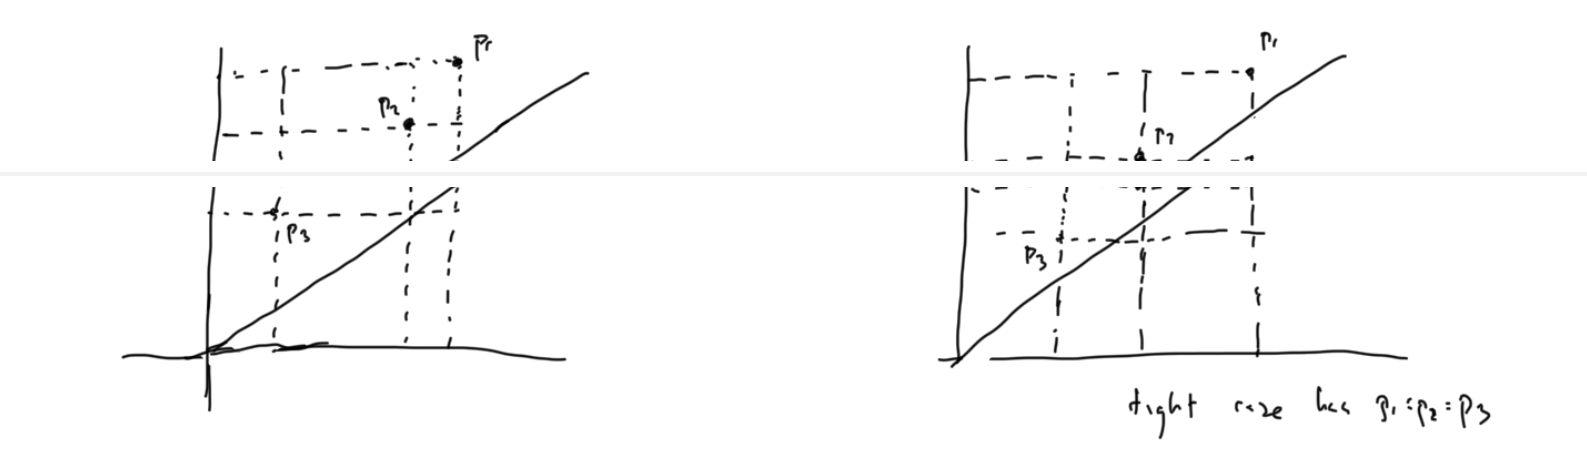
\includegraphics[width=\textwidth]{220103.png}
% \begin{tikzpicture}[scale=1.3]
%   \def\xmin{-1}
%   \def\xmax{3}
%   \def\ymin{\xmin}
%   \def\ymax{\xmax}
%   \draw[->] (\xmin,0) -- (\xmax,0) coordinate (x axis);
%   \draw[->] (0,\ymin) -- (0,\ymax) coordinate (y axis);
%   \draw (\xmin+.5,\ymin+.5) -- (\xmax,\ymax);
%   \node (origin) at (0,0) {};
%   \node (A) at (\xmax-1,\ymax-.3 ) {\textbullet $p_1$};
%   \node (B) at ($ (A) - (.8,.4)$) {\textbullet $p_2$};
%   \node (C) at ($ (A) - (1.3,1.5)$) {\textbullet $p_3$};
%  \foreach \startpoint [count=\i] in {(origin),(A),(B),(C)}{
%    \foreach \endpoint [count=\j] in {(origin),(A),(B),(C)} {
%      \ifnum \i < 5
%      \ifnum \j < 5
%      \draw[dotted] \startpoint -| \endpoint ;
%      % \draw[dashed] \endpoint -- \endpoint |- \startpoint;
%      % \draw[dashed] \startpoint -| \endpoint -- \endpoint;
%      \fi
%      \fi
%       }
%     }
%   \end{tikzpicture}
% \end{figure}
% \footnotesize{  The
%     distance between the atoms $p_1$ and $p_2$ is small relative to
%     their distances to the line $x=y$, so they contribute
%     $(p_1+p_2)^2$ to the mass of $\{x<y\}$ under the product of the
%     marginals. The distance between $p_1$ and $p_3$ is relatively
%     large, so they contribute only
%     $(p_1+p_3)^2-p_1p_3$.}
% \end{frame}

\begin{frame}
When $M=N=1$,
\begin{align}
  1-\sqrt{2(1-\aucpop)} \le \aucindiv \le \sqrt{2\aucpop}
\end{align}
 equivalently,
\begin{align}
  \frac{1}{2}\aucindiv^2 \le \aucpop \le 1 - \frac{1}{2}(1-\aucindiv)^2,\\
\end{align}

\begin{itemize}
\item When the personalized AUC is completely uninformative, $\aucindiv=1/2$,
the informativity of the population AUC is limited,
$1/8 \le \aucpop \le 7/8$.
\item However, when the population AUC is
  completely uninformative, $\aucpop=1/2$, the above bounds on the personalized AUC, which are tight, are vacuous, $0\le\aucindiv\le 1$.
% \item Situations where the population AUC $\to 1$ while the personalized AUC $\to 1/2$, may require some dependence between $M,N$ and $X,Y$
\end{itemize}
\end{frame}

\begin{frame}
  % In general, when $M$ and $N$ are each constant,
  \begin{theorem}\label{theorem:bounds}
    Let $(X,Y,M,N)\sim \P$ with $M=m$ and $N=n$  constant. Then
    \begin{align}
      \frac{1}{2}&\left(\aucindiv+\frac{\sum_{k,l}\P(X_{1k}=Y_{1l})}{2mn}\right)^2 \le \aucpop \\
      &\le 1-\frac{1}{2}\left(1-\aucindiv+\frac{\sum_{k,l}\P(X_{1k}=Y_{1l})}{2mn}\right)^2      
    \end{align}
    % [[drop 1 and 2 from X/Y observations in favor of primes throughout?]]
  \end{theorem}
  \begin{itemize}
\item Situations where the population AUC $\to 1$ while the personalized AUC $\to 1/2$, may require some dependence between $M,N$ and $X,Y$
\end{itemize}
\end{frame}

\section{Estimation}
\begin{frame}
 Let $\psi:V\times V\to\mathbb{R}$, $W=(X,Y,M,N)\sim\P$ with $(X,Y)\in V\times V$, $\psi\in L^2(\P)$, $M$ and $N$ counting numbers $> 0$ with finite means. Then:
  \begin{align}
    \sqrt{\I}(\aucpophat-\aucpop,\aucindivhat-\aucindiv) \leadsto \mathcal{N}(0,\Sigma)
  \end{align}
  with
  {\small
  \begin{align}
    \Sigma_{11} &= \lim_{\I\to\infty} \I\V(\hat\aucpop) =
    \E\left(\frac{\E(\Kernel_{12}\mid\W{1})+\E(\Kernel_{21}\mid\W{1})}{\E M\E N} - \aucpop\left(\frac{M_1}{\E M} + \frac{N_1}{\E N}\right)   \right)^2
    \\
    \Sigma_{22} &= \lim_{\I\to\infty} \I\V(\hat\aucindiv) =
    \V(\Kernel_{11}/(M_1N_1))
    \\
    \Sigma_{12} &= \lim_{\I\to\infty} \I\cov(\hat\aucpop,\hat\aucindiv) =
    \aucpop\E\left(\frac{\Kernel_{11}}{M_1N_1}\left(\frac{\Kernel_{12}+\Kernel_{21}}{\E\Kernel_{12}} - \frac{M_1}{\E M}-\frac{N_1}{\E N}  \right) \right)
  \end{align}
}  
  % $\sqrt{\I}(\aucpophat-\aucpop,\aucindivhat-\aucindiv) $ converges to a mean-zero bivariate normal distribution with covariance matrix given by
  % \begin{align}
  % \end{align}
% \end{theorem}
\end{frame}

\begin{frame}
  Simulation


  \begin{itemize}
  \item $M$ and $N$ are sampled as the negative and positive values in a correlated normal sample.
  \item The greater the correlation, the greater the imbalance between
    case and control observations within the clusters
  \end{itemize}
\end{frame}
\begin{frame}
  Two models for the observation vectors $(X,Y)$
  \begin{itemize}
  \item binormal model:
    \begin{align}
  (X,Y) \mid (M,N) \sim \mathcal{N}_{M+N}\left(
  % \begin{pmatrix}\mu_X\mathbbm{1}_M\\ \mu_Y\mathbbm{1}_N\end{pmatrix},
    \begin{pmatrix}0\cdot\mathbbm{1}_M\\ \Delta\cdot\mathbbm{1}_N\end{pmatrix},
            \begin{pmatrix} 1 & \rho & \cdots & \rho\\
              &\ddots &\ddots\\
              \rho & \cdots & \rho &1
            \end{pmatrix}
            \right)
\end{align}
\item   $\aucpop(P) = \Phi\left(\frac{\Delta}{\sqrt{2}}\right), \aucindiv(P) =  \Phi\left(\frac{\Delta}{\sqrt{2(1-\rho)}}\right)$
\item Censored binormal model: Sample $(\overline X,\overline Y)$, then clip the observations to $\pm a$


\end{itemize}
\end{frame}


\begin{frame}
  \begin{itemize}
\item Empirical power function of the test of $H_0:\aucpop=\aucindiv$ versus $\aucpop<\aucindiv$ using the
asymptotic estimator
\item  same as $H_0:|\aucpop-1/2|=|\aucindiv-1/2|,$ equal informativity
  \item normal data with and without clipping
\end{itemize}
\begin{figure}%[!tbp]
  \centering
  \subfloat{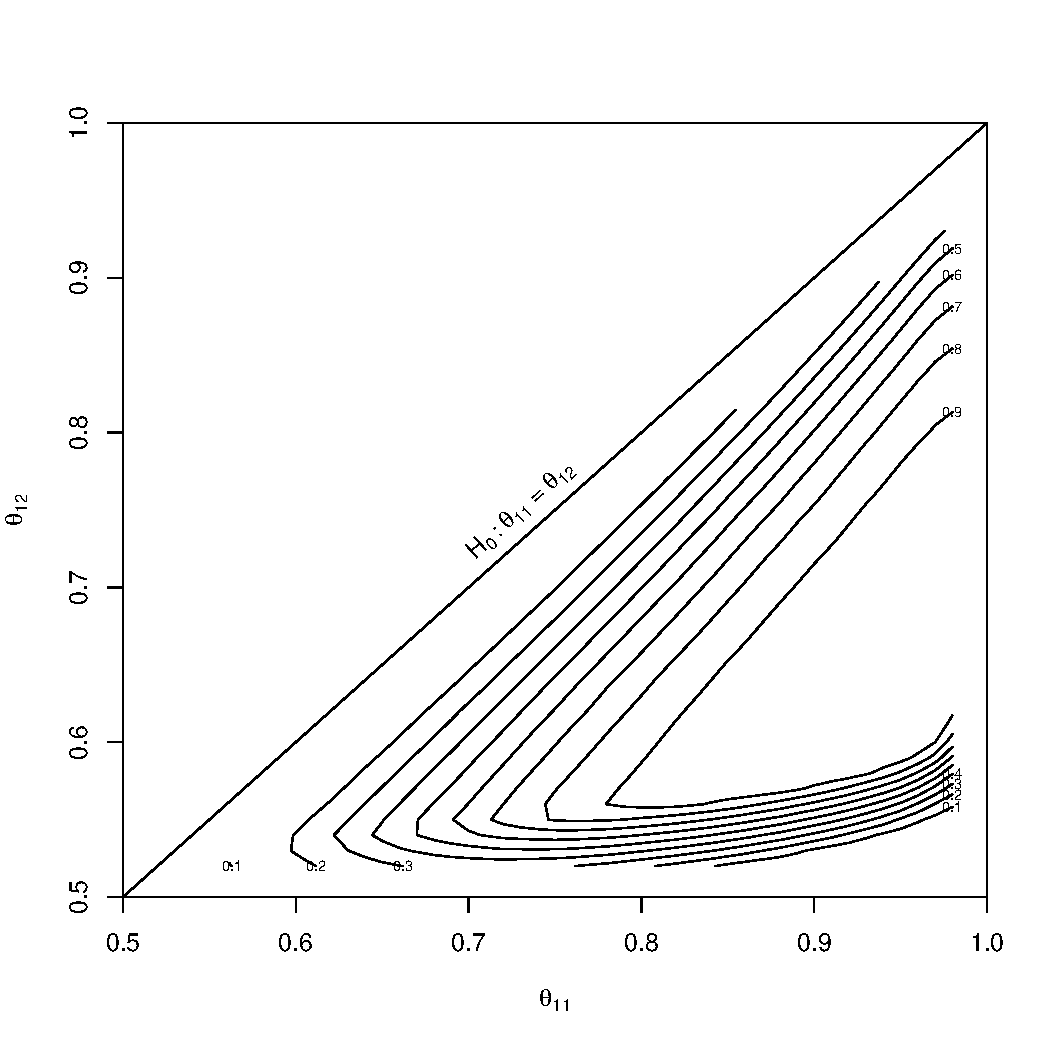
\includegraphics[width=0.5\textwidth]{../sim/220813/a/220813.pdf}}
  \hfill
  \subfloat{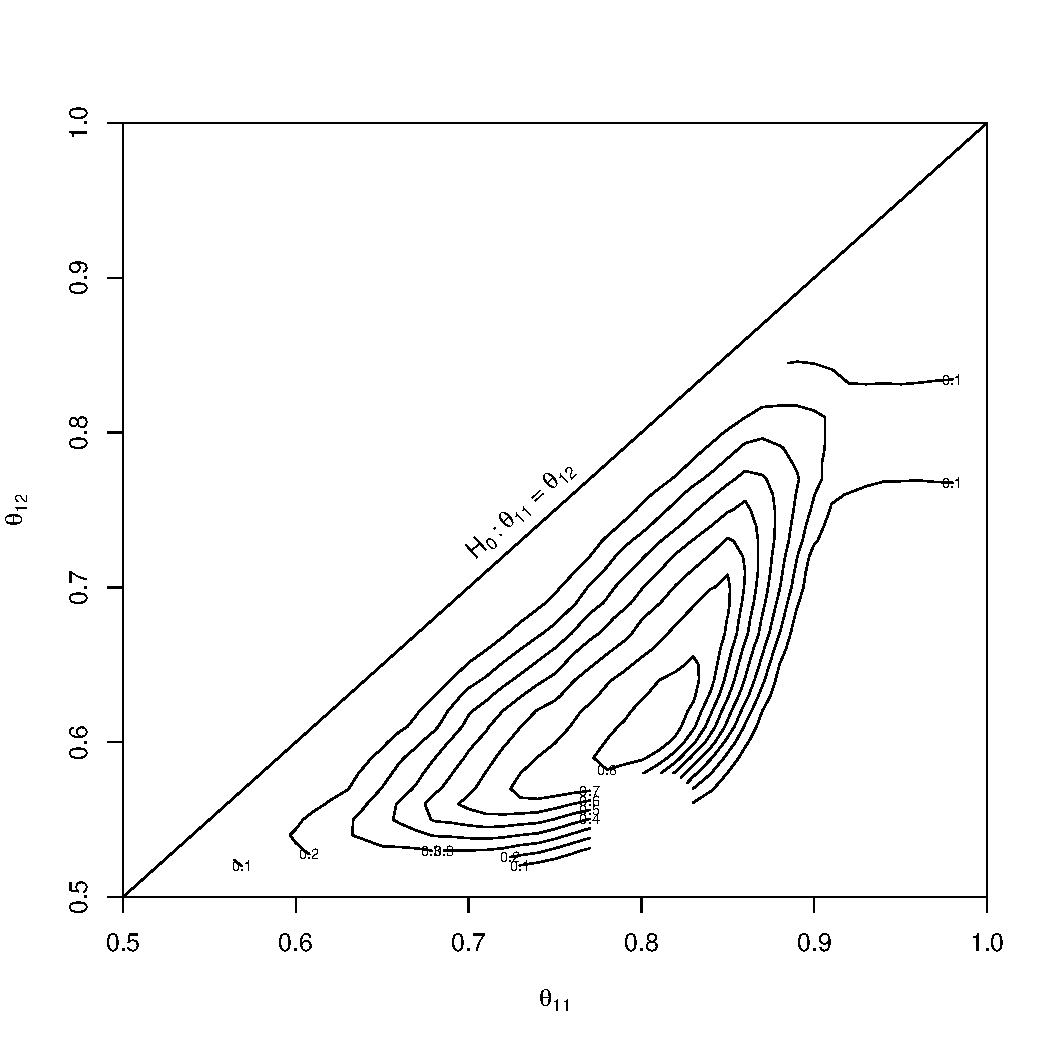
\includegraphics[width=0.5\textwidth]{../sim/220813/b/220813.pdf}}
  % \caption{}  \label{fig:power}
\end{figure}
\end{frame}


\section{Application}
\begin{frame}
  \begin{itemize}
  \item  The data consists of Terry stops in New York City and Boston.
  \item The analysis here focuses on the relationship between the duration of the
    stop and race of the suspect.
  \item We cluster the stops according to
    precinct, in the case of NYC, and according to the officer conducting
    the stop, in the case of Boston.
  \end{itemize}
\end{frame}

% begin{frame}
%     dkd
%   }
% \end{frame}

\begin{frame}
  \begin{table}
    % \resizebox{3cm}{!}{
    \small
    \addtolength{\tabcolsep}{-5pt}
    % \begin{tabular}{|l||C{3cm}|C{1cm}|C{1cm}||C{3cm}|C{1cm}|C{1cm}|}
  \hline
  & \multicolumn{3}{c||}{NYC} & \multicolumn{3}{c|}{Boston}\\
 \hline
 \hline
 group & mean duration (SD) & count & freq. & mean duration (SD) & count & freq.\\
 \hline
Asian & 14.24 (21.16) & 1139 & 0.02 & 25.00 (24.22) & 53 & 0.01 \\ 
  Black Hispanic & 11.01 (17.12) & 4675 & 0.09 & 15.28 (18.73) & 391 & 0.06 \\ 
  Black non-Hispanic & 10.99 (16.78) & 31588 & 0.58 & 19.06 (28.93) & 3448 & 0.55 \\ 
  White Hispanic & 11.21 (15.15) & 11486 & 0.21 & 15.63 (15.96) & 578 & 0.09 \\ 
  White non-Hispanic & 12.85 (16.18) & 4854 & 0.09 & 21.74 (33.01) & 1760 & 0.28 \\ 
  other & 11.84 (17.70) & 261 & 0.00 & 20.89 (23.90) & 93 & 0.01 \\ 
   \hline
\end{tabular}
       
\begin{tabular}{|l||C{2cm}|C{1cm}|C{1cm}||C{2cm}|C{1cm}|C{1cm}|}
  \hline
  & \multicolumn{3}{c||}{NYC} & \multicolumn{3}{c|}{Boston}\\
 \hline
 \hline
 group & mean duration (SD) & count & freq. & mean duration (SD) & count & freq.\\
 \hline
Asian & 14.24 (21.16) & 1139 & 0.02 & 25.00 (24.22) & 53 & 0.01 \\ 
  Black Hispanic & 11.01 (17.12) & 4675 & 0.09 & 15.28 (18.73) & 391 & 0.06 \\ 
  Black non-Hispanic & 10.99 (16.78) & 31588 & 0.58 & 19.06 (28.93) & 3448 & 0.55 \\ 
  White Hispanic & 11.21 (15.15) & 11486 & 0.21 & 15.63 (15.96) & 578 & 0.09 \\ 
  White non-Hispanic & 12.85 (16.18) & 4854 & 0.09 & 21.74 (33.01) & 1760 & 0.28 \\ 
  other & 11.84 (17.70) & 261 & 0.00 & 20.89 (23.90) & 93 & 0.01 \\ 
   \hline
\end{tabular}
    \caption{Summary estimates on the duration of Terry stops by racial group.\speak{boston data has black/white without hispanic coded; here blacks where ethnicity is not recorded or NA are grouped as black non-hisp. maybe do alternative analysis where those are all NA'd. boston data puts south asian with middle eastern, which is other here.}\speak{in the boston data about [[]] of the black or whtie observations have no recorded hispanic/non-hispanic status.}}
%}    % \label{table:data analysis:summary estimates}
\end{table}
\end{frame}

\begin{frame}
  $\aucpop < \aucindiv$
\begin{itemize}
  \item With Black race as the
  binary classification, the AUC analysis looks for a difference in
  location between the distribution of stop durations of non-Black
  (``control'') and Black (``case'') suspects.

  \item For the NYC data, the
  population AUC estimate is
  $\aucpophat=\input{input/da_black_nyc_theta12_mean.txt}$ with 95\%
  CI \input{input/da_black_nyc_theta12_CI.txt}\unskip, significantly
  different from the null value of $1/2$. The personalized AUC
  estimate is
  $\aucindivhat=\input{input/da_black_nyc_theta11_mean.txt}$ with a
  95\% CI \input{input/da_black_nyc_theta11_CI.txt}.

  \item A test of
  equality $H_0:\aucpop=\aucindiv$ against $\aucpop < \aucindiv$ returns a p-value of $.05\%$. The
  Boston data is similar.%  The population AUC estimate is
  % \input{input/da_black_boston_theta12.txt} and the personalized AUC estimate
  % is \input{input/da_black_boston_theta11.txt}. A test of equality
  % $H_0:\aucpop=\aucindiv$ against $\aucpop < \aucindiv$ returns the p-value $.91\%$. Confidence
  % ellipses are plotted in Figure \ref{fig:data analysis:confidence
  % ellipses}.
\end{itemize}
\speak{  
  The data recalls the situation depicted in
  Fig. \ref{fig:comparison:b}, though of course the difference between
  the two AUCs is less dramatic here than in the artificial example
  constructed there.
}
\end{frame}

\begin{frame}
  \centering
  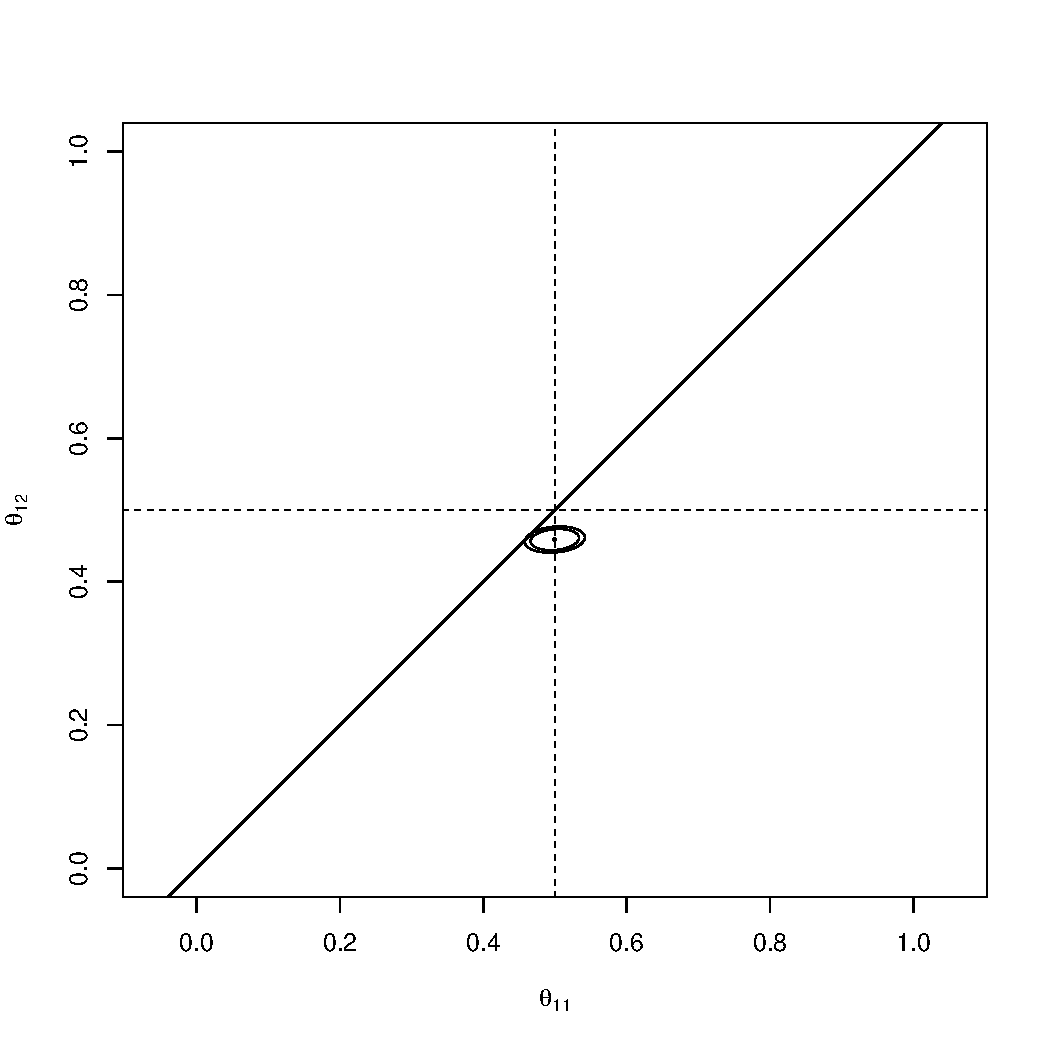
\includegraphics[width=0.5\textwidth]{220823_nyc.pdf}
  \end{frame}
  
\begin{frame}
  $\aucindiv < \aucpop$

  \begin{itemize}
    \item For the Boston data, the personalized
  AUC, \input{input/da_white_boston_theta11.txt}\unskip, is more
  informative than the population AUC,
  \input{input/da_white_boston_theta12.txt}\unskip,
  \item the test of
  equality versus $\aucindiv < \aucpop$ returning a p-value of
  % \input{input/da_white_boston_pval.txt}
  2.5\%.
\end{itemize}
\speak{This
  analysis therefore corresponds to the situation in...}
\end{frame}

\begin{frame}
  No significant difference between $\aucpop$ and
  $\aucindiv$.
\begin{itemize}
  \item duration of the stop between
  non-Hispanic (``control'') and Hispanic (``case'') suspects: For both the NYC and Boston data, neither the population AUC nor
  personalized AUC is significantly different from the null value
  $1/2$, and the test of equality of the two AUCs fails to reject.

\item For the Boston data, whether one takes the case status to be
  non-Hispanic Black or non-Hispanic White, the two AUCs are
  statistically indistinguishable from each other and each is
  indistinguishable from the null value $1/2$.
\end{itemize}
\speak{many other examples since this is the null situation}
\end{frame}

\begin{frame}
  Haben Michael, Lu Tian. The Population and Personalized AUCs. Forthcoming. Available at: \texttt{https://haben-michael.github.io/}\\
  \vspace{.7in}
  \centering
\end{frame}

\end{document}
